%-----------------------------------------------------
% index key words
%-----------------------------------------------------
\index{geometry}

%-----------------------------------------------------
% name, leave blank
% title, if the exercise has a name i.e. Hilbert's matrix
% difficulty = n, where n is the number of stars
% origin = "\cite{ref}"
%-----------------------------------------------------
\begin{Exercise}[
name={},
title={}, 
difficulty=0,
origin={\cite{SM}}]\label{quadParallelogram}
Prove that the quadrilateral $PQRS$, whose vertices are the midpoints of the sides of an arbitrary quadrilateral $ABCD$, is a parallelogram.
    \begin{center}
        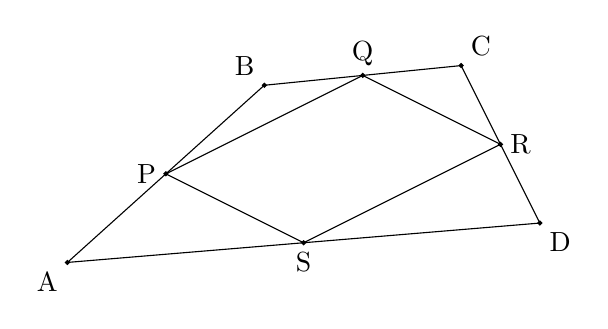
\begin{tikzpicture}
            \draw (0,0) -- (2.5,2.25) -- (5,2.5) -- (6,0.5) -- (0,0);
            \draw[fill] (0,0) circle [radius = 0.025];
            \draw[fill] (2.5,2.25) circle [radius = 0.025];
            \draw[fill] (5,2.5) circle [radius = 0.025];
            \draw[fill] (6,0.5) circle [radius = 0.025];
            \draw[fill] (1.25,1.125) circle [radius = 0.025];
            \draw[fill] (3.75,2.375) circle [radius = 0.025];
            \draw[fill] (5.5,1.5) circle [radius = 0.025];
            \draw[fill] (3,0.25) circle [radius = 0.025];
            \draw (1.25,1.125) -- (3.75,2.375) -- (5.5,1.5) -- (3,0.25) -- (1.25,1.125);
            \node [below left] at (0,0) {A};
            \node [above left] at (2.5,2.25) {B};
            \node [above right] at (5,2.5) {C};
            \node [below right] at (6,0.5) {D};
            \node [left] at (1.25,1.125) {P};
            \node [above] at (3.75,2.375) {Q};
            \node [right] at (5.5,1.5) {R};
            \node [below] at (3,0.25) {S};
        \end{tikzpicture}
    \end{center}

\end{Exercise}

\begin{Answer}
Use Exercise \ref{chordOfTriangle} twice.
\end{Answer}
